Voici un problème classique des manuels scolaires de mathématiques pour collégiens ou lycéens français. Imaginons la situation suivante où M. CITER
\footnote{
	\emph{\og citer \fg} est l'anagramme de \emph{\og recti \fg} pour \emph{\og rectiligne \fg} comme les représentations sur le schéma.
}
doit amener, à l'aide d'un sceau, de l'eau de la rivière à l'abreuvoir pour ses moutons qui sont dans un enclos.

\smallskip
\begin{center}
	\fbox{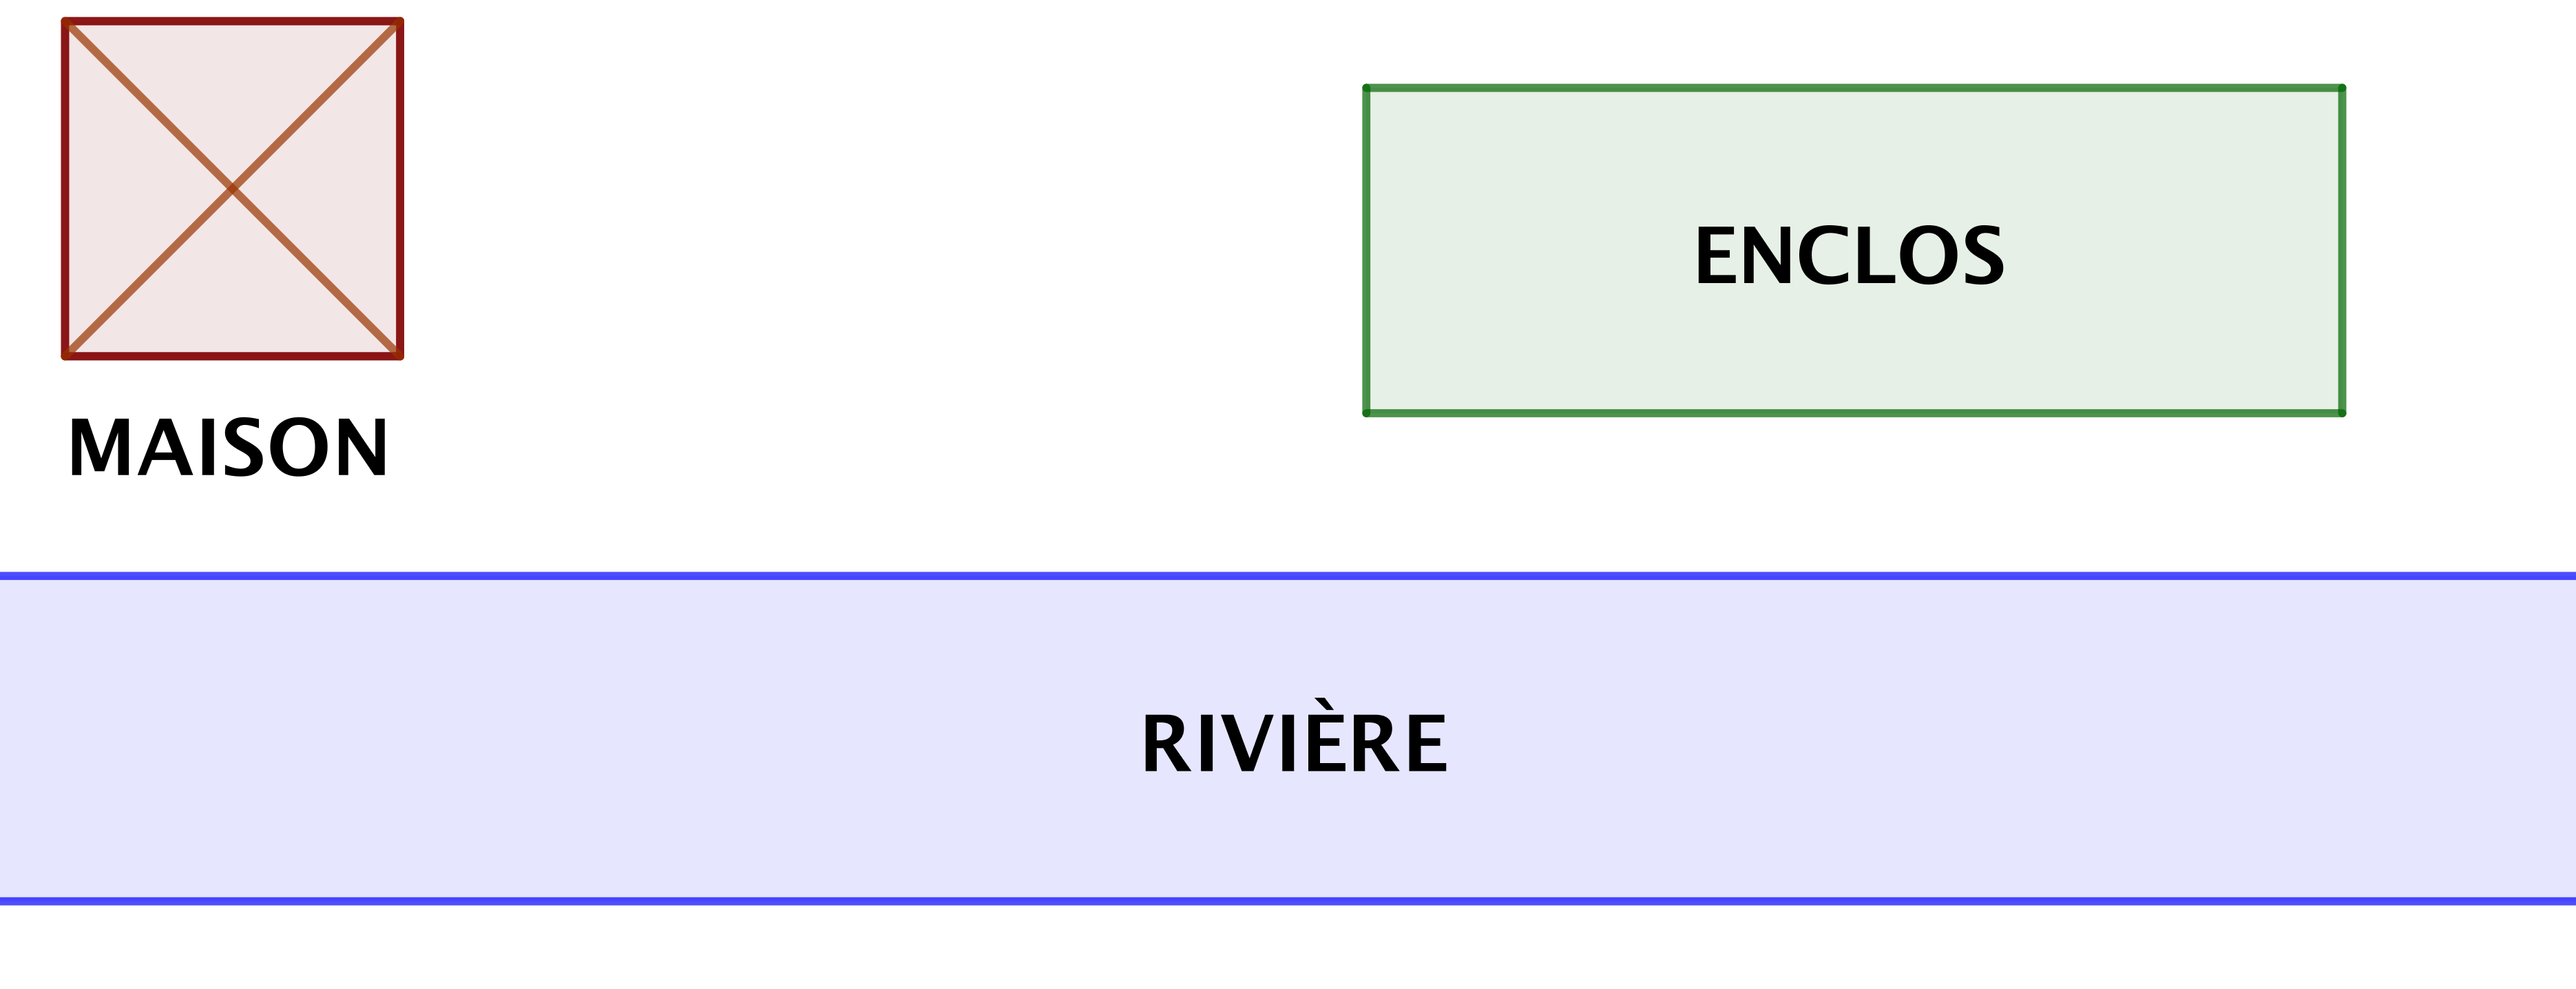
\includegraphics[scale = .6]{river-pb.png}}
\end{center}


\medskip


Commençons par simplifier un tout petit peu les données en ne gardant que la rive à laquelle M. CITER peut accéder

\smallskip
\begin{center}
	\fbox{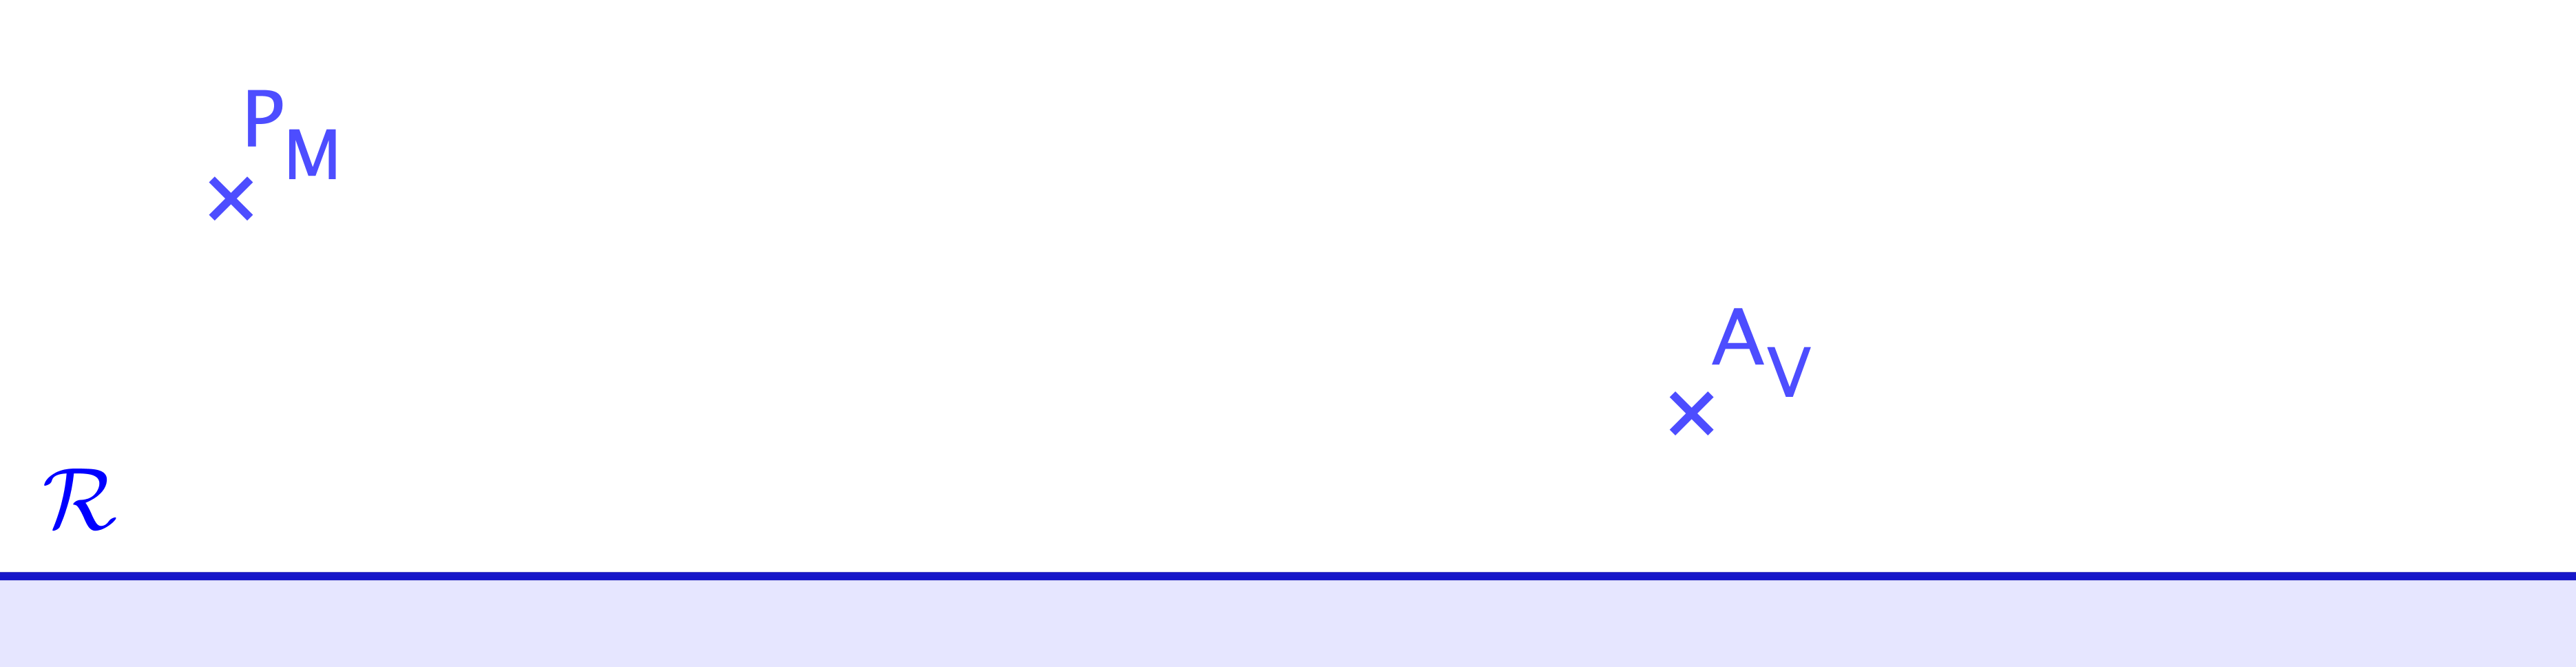
\includegraphics[scale = .6]{river-pb-simplified.png}}
\end{center}


\medskip


Un première solution consistèe à chercher le chemin le plus court pour accéder à $A_V$ depuis $P_M$ en bassant par la rive $\probaset{R}$

Ce problème a une solution géométrique très simple que voici
\footnote{
	Il existe une réponse analytique via l'étude des extrema d'une fonctions omme de longuer. Le point délicat est d'avoir un théorème d'existence de minimum car le signe de la dérivée n'est pas évident à déterminer.
}.

\smallskip
\begin{center}
	\fbox{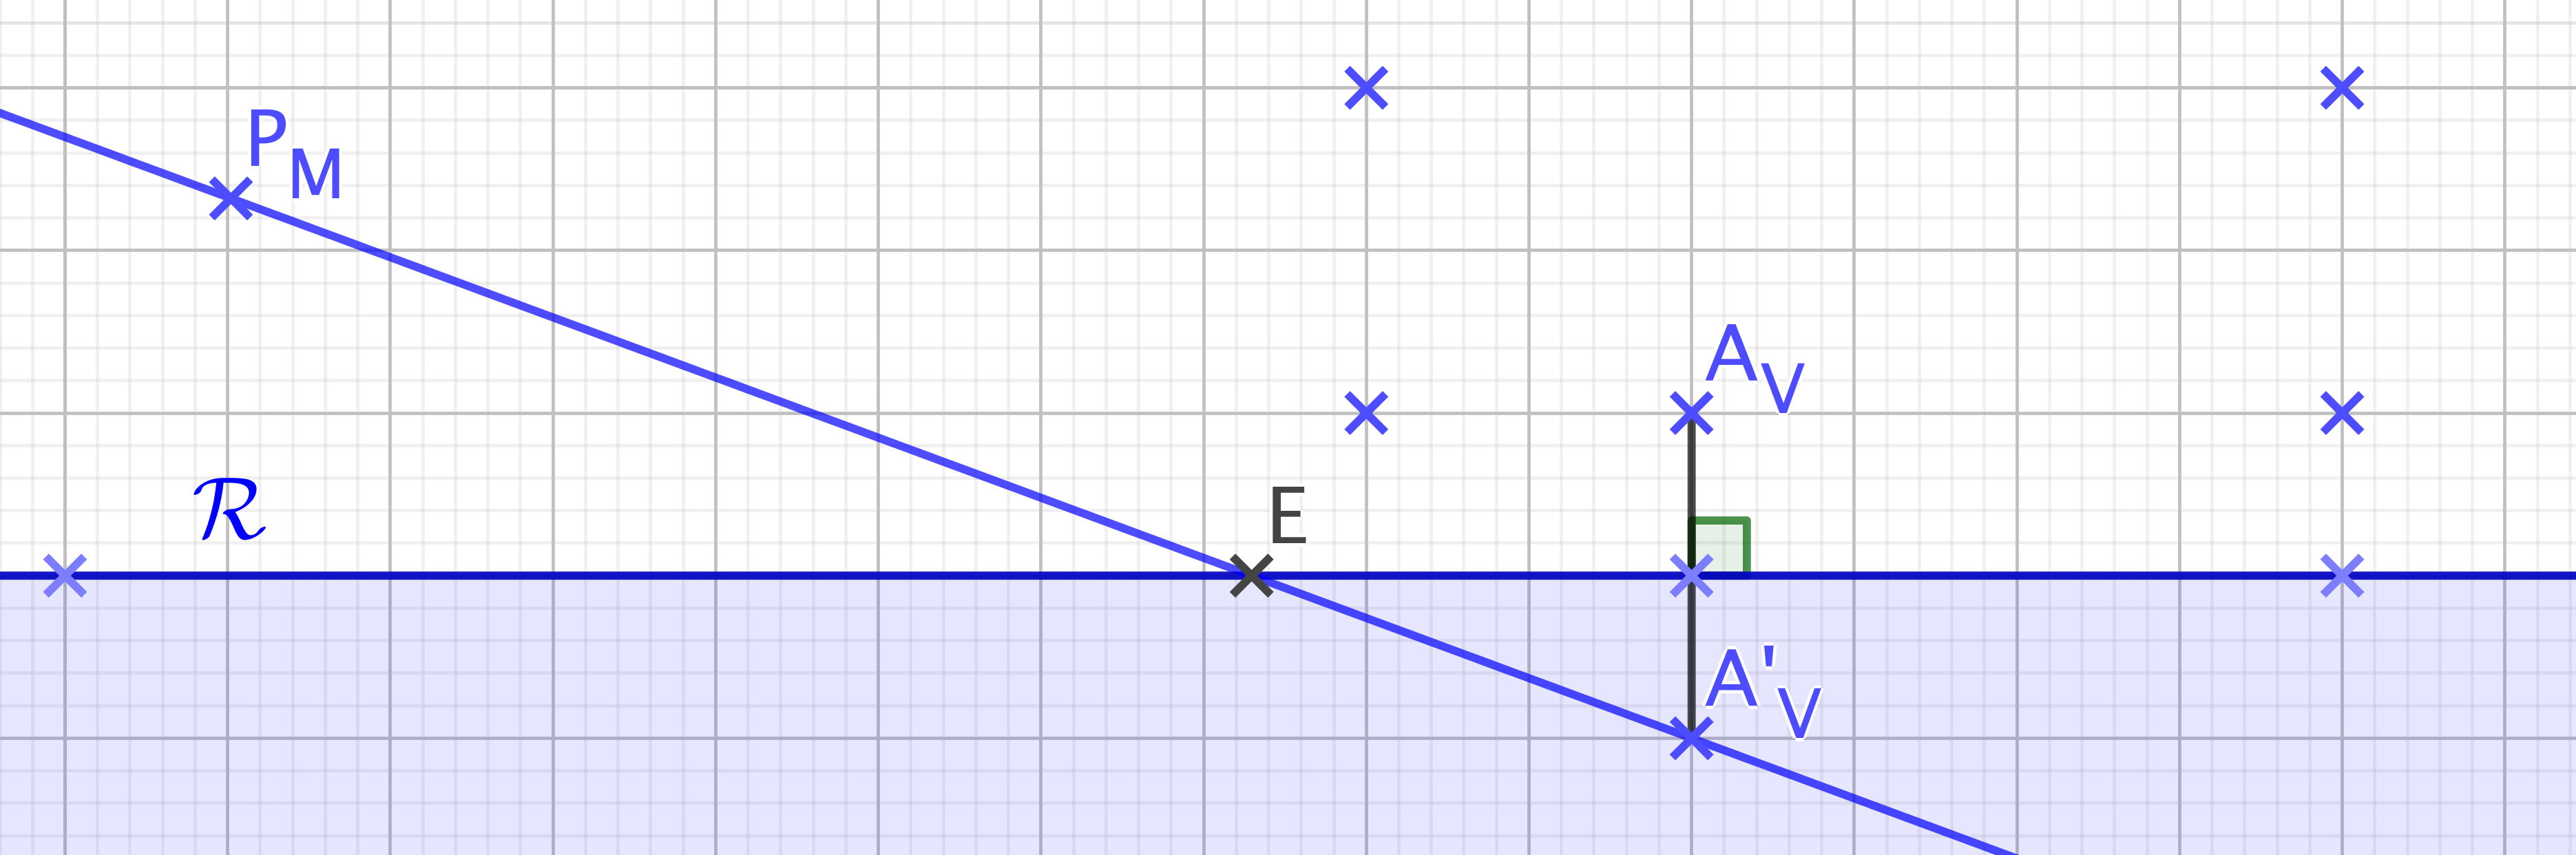
\includegraphics[scale = .6]{river-pb-geo-sol.png}}
\end{center}


\medskip


Très jolie solution mais elle ne tient pas compte de l'effort à fournir pour amenr le seau d'eau lourd à porter, ou bien que faire si 'lon doit utiliser plusieurs e-seaux ??? Avec cette contrainte en ttpete, la solutione st immédiat. La voici.

\smallskip
\begin{center}
	\fbox{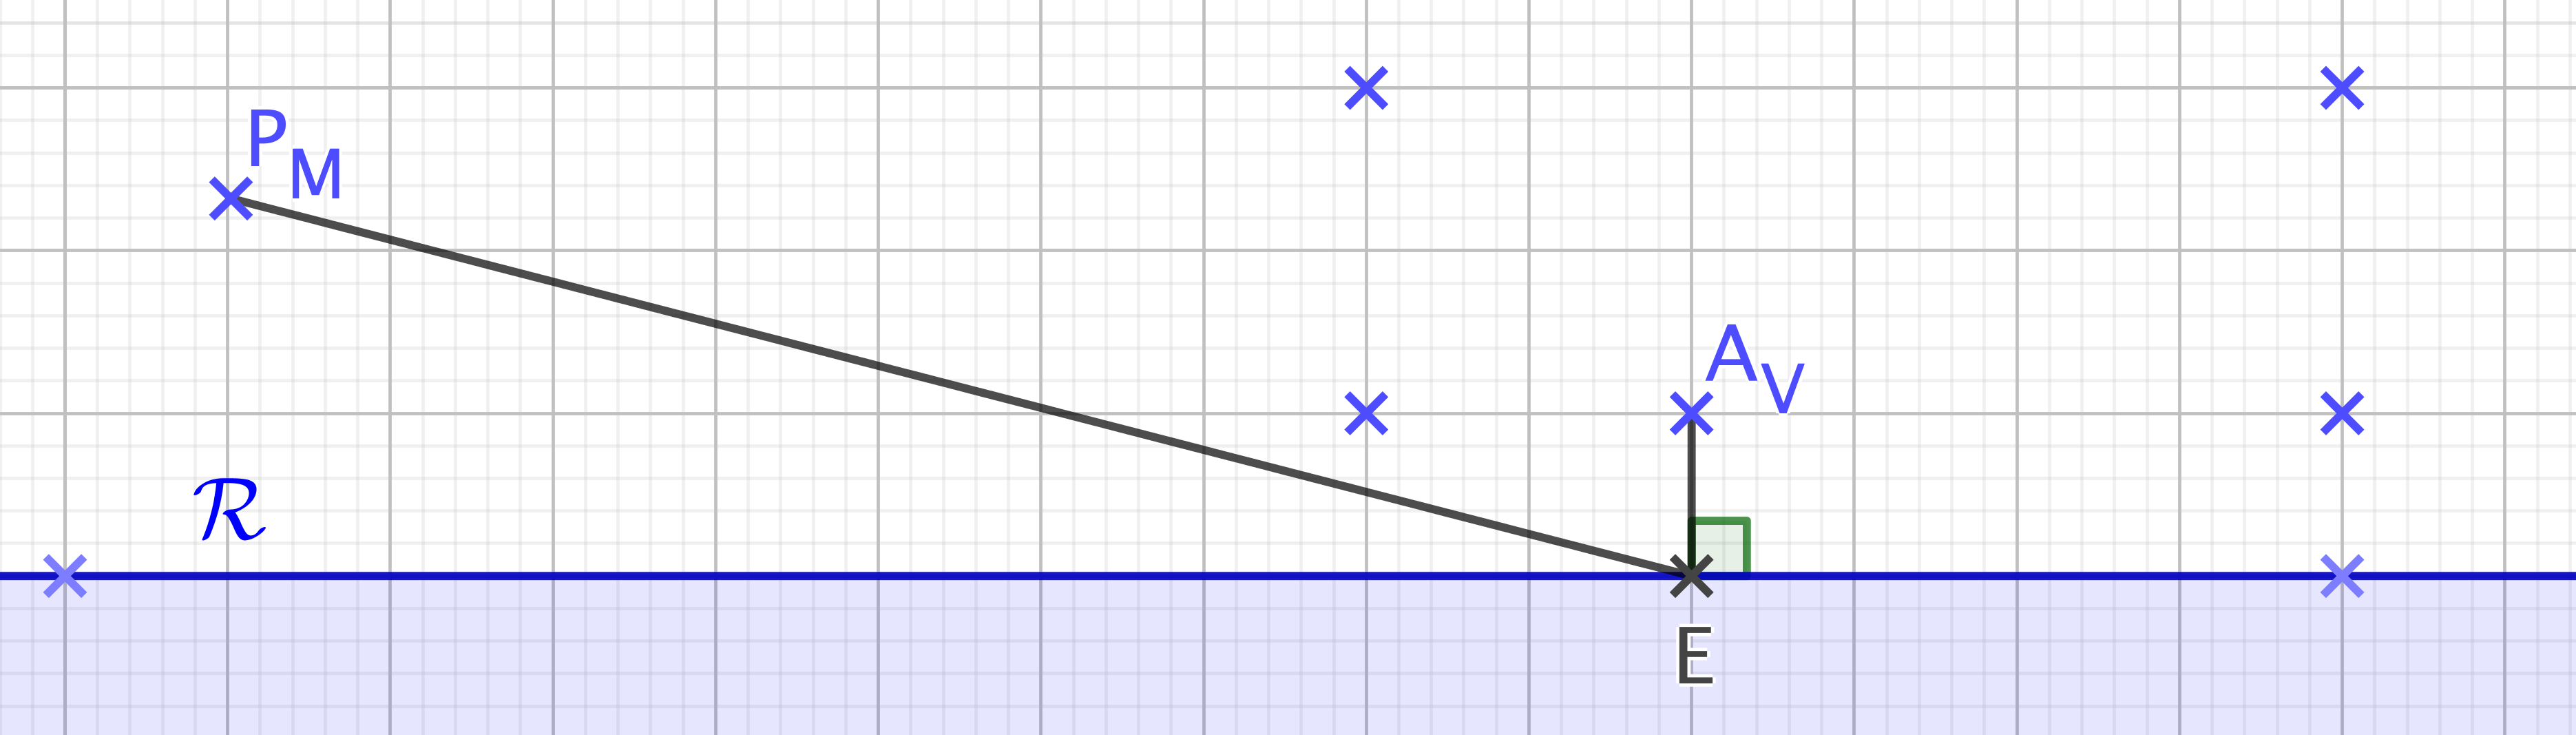
\includegraphics[scale = .6]{river-pb-practical-sol.png}}
\end{center}


\medskip


???? 
